%%%%%%%%%%%%%
%
%
% Text for dissertation appendix B and the signal chain response white paper.  
% They will have identical text.
%
% Ben Rotter - University of Hawaii at Manoa - March 2017
%
%%%%%%%%%%%%%%


	The generation of a system impulse response for the ANITA3 instrument from pre-flight calibration measurements is required to accurately relate the digitized time series of analog voltages propagated to the detector electronics to the correlating electric field physically transiting the instrument.  As the system is sensitive to a wide bandwidth, a full frequency dependent array of complex phasors is required to completely characterize the system.  The ANITA3 (and more recent ANITA4) flights employ slightly different antennas than the previous ANITA1 and ANITA2 flights whose purpose is to capture additional sub 200MHz frequency electromagnetic signals. Additionally, the amplification and filtering chains of the newer flights have subtle modifications preclude direct relation between their results and those of earlier flights.  This change necessitates a thorough analysis and characterization of the full ANITA3 signal chain, from antenna to digitizer.
	
\section{Introduction}

	There are two distinct systems on the ANITA3 instrument that alter the received time domain signal on its to the digitizer: the Seavey horn antennas, and the filtering and amplification network colloquially known as the signal chain.  The antennas used on the ANITA flight are broad band, with a design bandwidth of 180MHz to 1200MHz, whose dual orthogonal polarizations have co-located phase centers.  These antennas couple the propagating electromagnetic (EM) radiation emitted by an extensive comic ray or neutrino air shower (EAS) into a 50$\Omega$ transmission line by uniformly transforming the impedance from that of free space to that of the RF system.  The collection of amplifiers, filters, and other 50-ohm RF components that populate the path between the antenna and the LABRADOR chip is known as the signal chain, and adds additional frequency dependent gain and phase modulation before finally being read out by a fast sampling broad band ADC.  To calibrate these two systems, input signals were injected into the systems and measurements were taken of both the input and output signal on a calibrated oscilloscope.  The methods and techniques used to generate an impulse response using these input and output signals will be discussed, as well as the results for the ANITA3 flight.

\subsection{Discrete Fourier Transform}

	To determine the spectral content of a time domain signal, I have employed the use of a Discrete Fourier Transform (DFT).  Equation \ref{eqn:DFT} exhibits a transformation between a discretely sampled time domain signal $x_{n}(t)$ and the equivalent Fourier series $\mathcal{F}_{k}(f)$.  Additionally, equation \ref{eqn:IDFT} shows the inverse of the DFT, with a $\frac{1}{N}$ normalization to preserve reciprocity of the transformations.

\begin{equation}
\mathcal{F}_{k} = \sum_{n=0}^{N-1} x_{n}e^{-2\pi ikn/N}
\label{eqn:DFT}
\end{equation}

\begin{equation}
x_{n} = \frac{1}{N}\sum_{k=0}^{N-1} \mathcal{F}_{k}e^{-2\pi ikn/N}
\label{eqn:IDFT}
\end{equation}

As our measured signal is required to be purely real, the Fourier equivalent series will be hermitian, setting the limits for the sum to purely positive integers.  Additionally, though a true Fourier transform takes the time or frequency integral over its respective range and thus introduces a time multiplication to the result, the DFT does not have a time normalization, leaving the units of both arrays as Volts.

The effect of transforming from a time series to a Fourier series and back should be zero, however any signal manipulations such as zero padding, up sampling, or truncating, will have an effect on the opposing Fourier equivalent pair as well.  This can be used to manipulate signals in a manner that matches the physical boundaries of the system.


\subsection{Units and Spectrum Discussion}

	Accurately representing the amount of power in a time domain waveform or network as a function of frequency requires both a normalized Fourier transform that obeys Parseval's Theorem, as well as the appropriate units.  There are two main types of signals which we are considering in this analysis, absolute measurements, referenced to a measured voltage on constant impedance network, and relative measurements relating two different measured signals.  
	
	An example of an absolute measurement is the time series waveforms captured on oscilloscopes.  These can be described by decibles referenced to 1mW (dBm), seen in Equation \ref{eqn:dBm}, or Power Spectral Density (PSD), represented by dBm/Hz and seen in Equation \ref{eqn:PSD}.  For the purposes of this analysis, the Power Spectral Density will be used.
	
\begin{equation}
Power(f) = 10log_{10}(\frac{|\mathcal{F}(f)|^{2} * 1000[\frac{mW}{W}]} {Z})\qquad [dBm]
\label{eqn:dBm}
\end{equation}

	
\begin{equation}
PSD(f) = 10log_{10}(\frac{|\mathcal{F}(f)|^{2} * 1000[\frac{mW}{W}]} {Z*df})\qquad [dBm/Hz]
\label{eqn:PSD}
\end{equation}

	
	An example of relative measurements are network analyzer S21 measurements and transfer functions, which do not quantify an absolute power, only a ratio of powers.

	The ratio of spectral power between two different signals $x_{A}(t)$ and $x_{B}(t)$, can be done through division of their equivalent Fourier representations $\mathcal{F}_{A}(f)$ and $\mathcal{F}_{B}(f)$.  The logarithmic magnitude of this ratio is what is most often recognized as the gain of the network between the two measured signals.  The calculation of the gain is seen in Equation \ref{eqn:gain}
	
\begin{equation}
Gain(f) = 10log_{10}(|\frac{\mathcal{F}_{A}(f)}{\mathcal{F}_{B}(f)}|^{2}) \qquad [dB]
\label{eqn:gain}
\end{equation}


	Note that the subtraction of an absolute measurement, regardless of normalization, yields a gain.


\section{Seavey Broad Band Quad-ridge Antenna Impulse Response}

	\subsection{Measurement Goals}

	Many calibration measurements were taken for the antennas used in the ANITA3 flight.  Each measurement probed a different characteristic of the antennas, and had various drawbacks and benefits.  There are several major parameters of interest for the antenna measurements. First, the absolute phase and gain response for any incident EM field at the peak response angle.  This angle of peak response, nominally pointed orthogonally to the antenna face, is known as the "boresight" angle, and the resulting quantity is known as the antenna gain. The directionality and gain pattern as a function of angle off the maximal transmission and receive direction is directly related to the antenna gain, and is needed to determine amplitudes for off signals incident at angles away from the bore sight.   Lastly, a measurement of the cross polarization fraction is required to determine the full Stokes parameters of any incident field.
	
	\subsection{Measurements Summary}
	
	The three different measurements were taken that are discussed in this paper, each of which probe a unique region of the full calibration measurement.  
	
		\subsubsection{UH Anechoic Chamber}
		First, a measurement was taken at the University of Hawaii at Manoa in a copper lined, RF sealed, anechoic chamber using two "identical" (same model and manufacturing batch) ANITA3 flight antennas.  This measurement allowed a maximally noise free environment in which to measure any small signal effects that may be present in the antennas.  It also removes the requirement for correlation and averaging of multiple waveforms, decreasing uncertainty introduced by interpolation techniques.  Unfortunately, the size of the anechoic chamber forced the distance between the antennas into the near field region for the lower side of the frequency bandwidth.  This causes results below 200MHz, with a wavelength of ~1.6m and minimum far field distance requirement of 3.2m, to be slightly distorted and require a 	Fresnel correction. As this is the region in which the antennas were supposed to perform differently than previous ANITA antenna designs, this experimental setup and required correction is highly problematic.  Additionally, measurements of the gain pattern far off the maximal bore-sight angle have Fresnel zones occluded by the absorbing material that lined the walls of the chamber, once again introducing Fresnel interference and increasing the uncertainty in the measurements.
	
		\subsubsection{UH Rooftop Measurements}
	Additional tests were undertaken at the University of Hawaii with much larger separation distances.  To accomplish this, the two antennas under test were placed on building rooftops separated by a moderately sized courtyard.  The building separation was large enough to escape the near-field of the lower frequency antenna response, yet close enough to preclude any ground bounce interference or multi-path issues.  These measurements were plagued by anthropogenic noise, however a large sample of waveforms uncorrelated to this noise was taken reducing the resulting background significantly.  These measurements provide the best results for the absolute system gain and antenna directivity.
	
		\subsubsection{Palestine TX 2014 Antenna Consistency Checks}
	Finally, for the full ANITA flight the consistency and similarity of all 48 antennas needed to be measured.  Bore-sight gain measurements were taken for all antennas at the Columbia Scientific Balloon Facility (CSBF) in Palestine TX during the 2014 integration campaign of the ANITA3 payload.  This was done in a CSBF balloon hangar, and is detailed in the following section
	
	
	
	\subsection{Absolute Boresight Complex Antenna Height}
		
		The relationship between the magnitude of an electric field vector and the induced potential on the transmission line output of the antenna is a combination of the radiation efficiency and beam pattern, and is colloquially known as the complex antenna height, measured in units of volts per meter, and represented in this paper by $\mathcal{H}_{ant}$.
		
		
	The equation for determining the complex antenna height of an antenna receiving an impulse in a transceiver pair, where the transmission antenna's height is known, is given by Equation \ref{eqn:antHeight}.
	
\begin{equation}
\mathcal{H}_{Rx}(f) = \frac{ c r(f) \mathcal{F}_{rec}(f)}{ if \mathcal{F}_{src}(f) \mathcal{H}_{Tx}(f) } 
\label{eqn:antHeight}
\end{equation}

In this equation, $f$ is the radiation frequency, $\mathcal{H}(f)$ represents the complex antenna height of the receive (Rx) and transmit (Tx) antennas, $c$ is the speed of light, $\mathcal{F}(f)$ is the Fourier equivalent of the time sampled waveform for the source (src) and received (rec) impulse, and $r(f)$ is the free space path distance between the phase centers of the antennas.  

The location of the phase centers as a function of antenna geometry were not known prior to this analysis, and would require additional absolute timing measurements.  For the purposes of this analysis a linear relationship between frequency and phase center was derived assuming two points: the 180MHz phase center is at the antenna face, and the 1.2GHz phase center was at the feed point.  The distance between the antenna face and the feed point is 21.86" for the vertically polarized channel, and 22.65" for the horizontally polarized channel, as seen in Figure \ref{fig:antDim}

	
\begin{figure}
\centering
	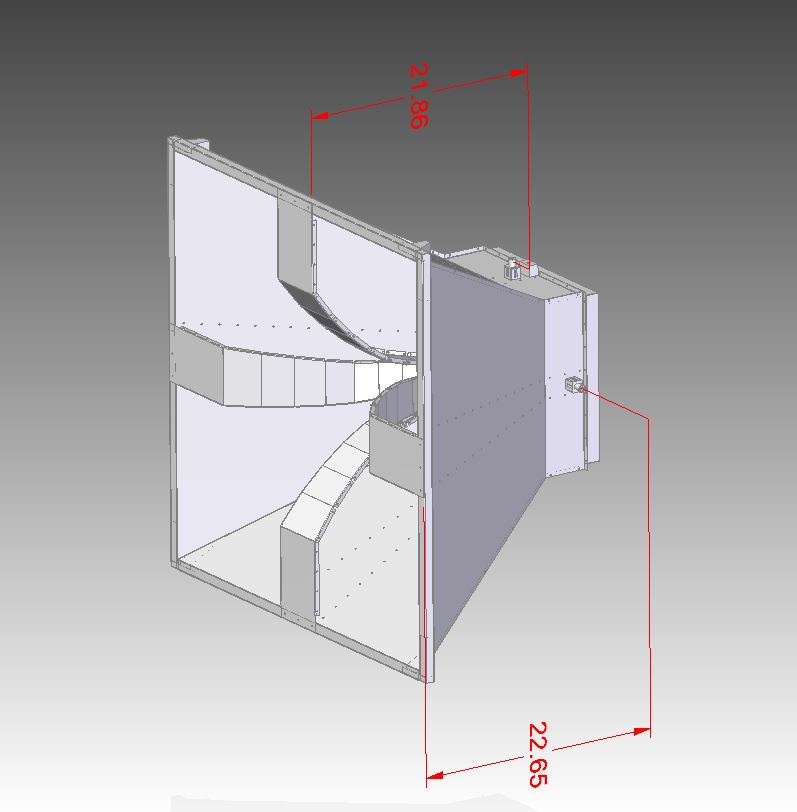
\includegraphics[width=0.7\textwidth]{../figures/ANITA_HORN_FEED_DIM}
	\caption{CAD model of the Seavey quad ridge horn antenna.  The distance between the face of the antenna and the feed point is annotated for use in estimating the phase center location as a function of frequency.}
\label{fig:antDim}
\end{figure}



If the antennas are identical, i.e $\mathcal{H}_{Rx}(f) = \mathcal{H}_{Tx}(f)$, Equation \ref{eqn:antHeight} becomes:

\begin{equation}
\mathcal{H}_{ant}(f) = \sqrt{ \frac{c r(f)}{if} \frac{\mathcal{F}_{rec}(f)}{\mathcal{F}_{src}(f)} } \\
\label{eqn:antHeight2}
\end{equation}

Note that using Equation \ref{eqn:antHeight2} results in a sign degeneracy as there are two possible solutions that satisfy the square root term.  This manifests itself as a lack of constraint on the absolute polarity of the emitted signal.  Determining the absolute polarity of the antennas requires using a calibrated reference antenna of which the polarity is previously known.


Complex antenna height relates electric field to measured voltage according to the following equation:

\begin{equation}
\frac{V_{rec}(t)}{\sqrt{Z_{sys}}} = h(t) \circ \frac{ E_{rad}(t) }{ \sqrt{Z_{o}} } \\
\label{eqn:antHeight2EField}
\end{equation}

Where $\circ$ is the convolution operator, $Z_{sys}$ is the matched impedance of the transmission line (50$\Omega$ in our system) and $Z_{o}$ is the impedance of free space (377$\Omega$).


	\subsection{Antenna Gain}
		The figure of merit for the absolute radiative power of an an antenna is called the Antenna Gain, and is calculated by taking the logaritm of the ratio between the measured peak radiated power of the antenna under test and that of an isotropically emitting antenna.  This value takes on the units dBi.  The equation to determine the antenna gain from the normalized complex antenna height is shown in equation \ref{eqn:antGain}.
		
\begin{equation}
G_{eff}(f) =  \frac{4\pi f^{2}}{c^{2}} | \mathcal{H}_{ant}(f)|^{2}
\label{eqn:antGain}
\end{equation}

	\subsection{Results of Palestine Antenna Measurements}
	
		All 48 antennas for the ANITA3 flight were measured at the Columbia Scientific Balloon Facility (CSBF) in Palestine, TX during the 2014 integration campaign.  The complex antenna height did not vary between antennas, and resulted in an average antenna gain of approximately 10dBi.  Figures \ref{fig:antennaGain} through \ref{fig:antResponse_fftV} show the results for all antennas.
		

\begin{figure}
\centering
\makebox[\textwidth]{%
	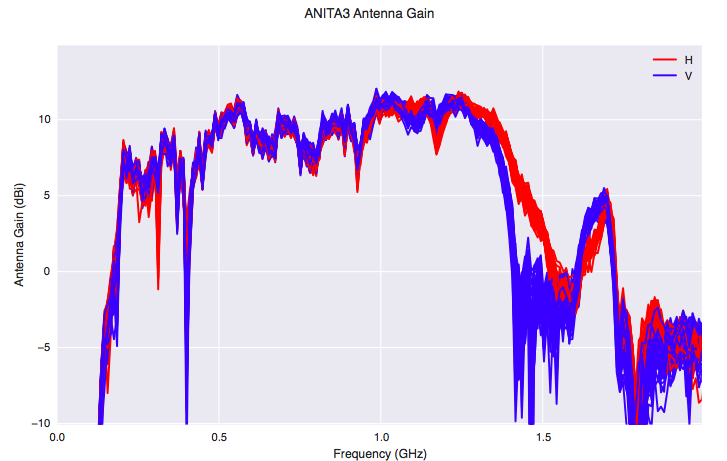
\includegraphics[width=1.5\textwidth]{../figures/antennaGain} }
	\caption{Results for the antenna gain as a function of frequency for all 48 ANITA3 horn antennas.}
\label{fig:antennaGain}
\end{figure}

\begin{figure}
\centering
\makebox[\textwidth]{%
	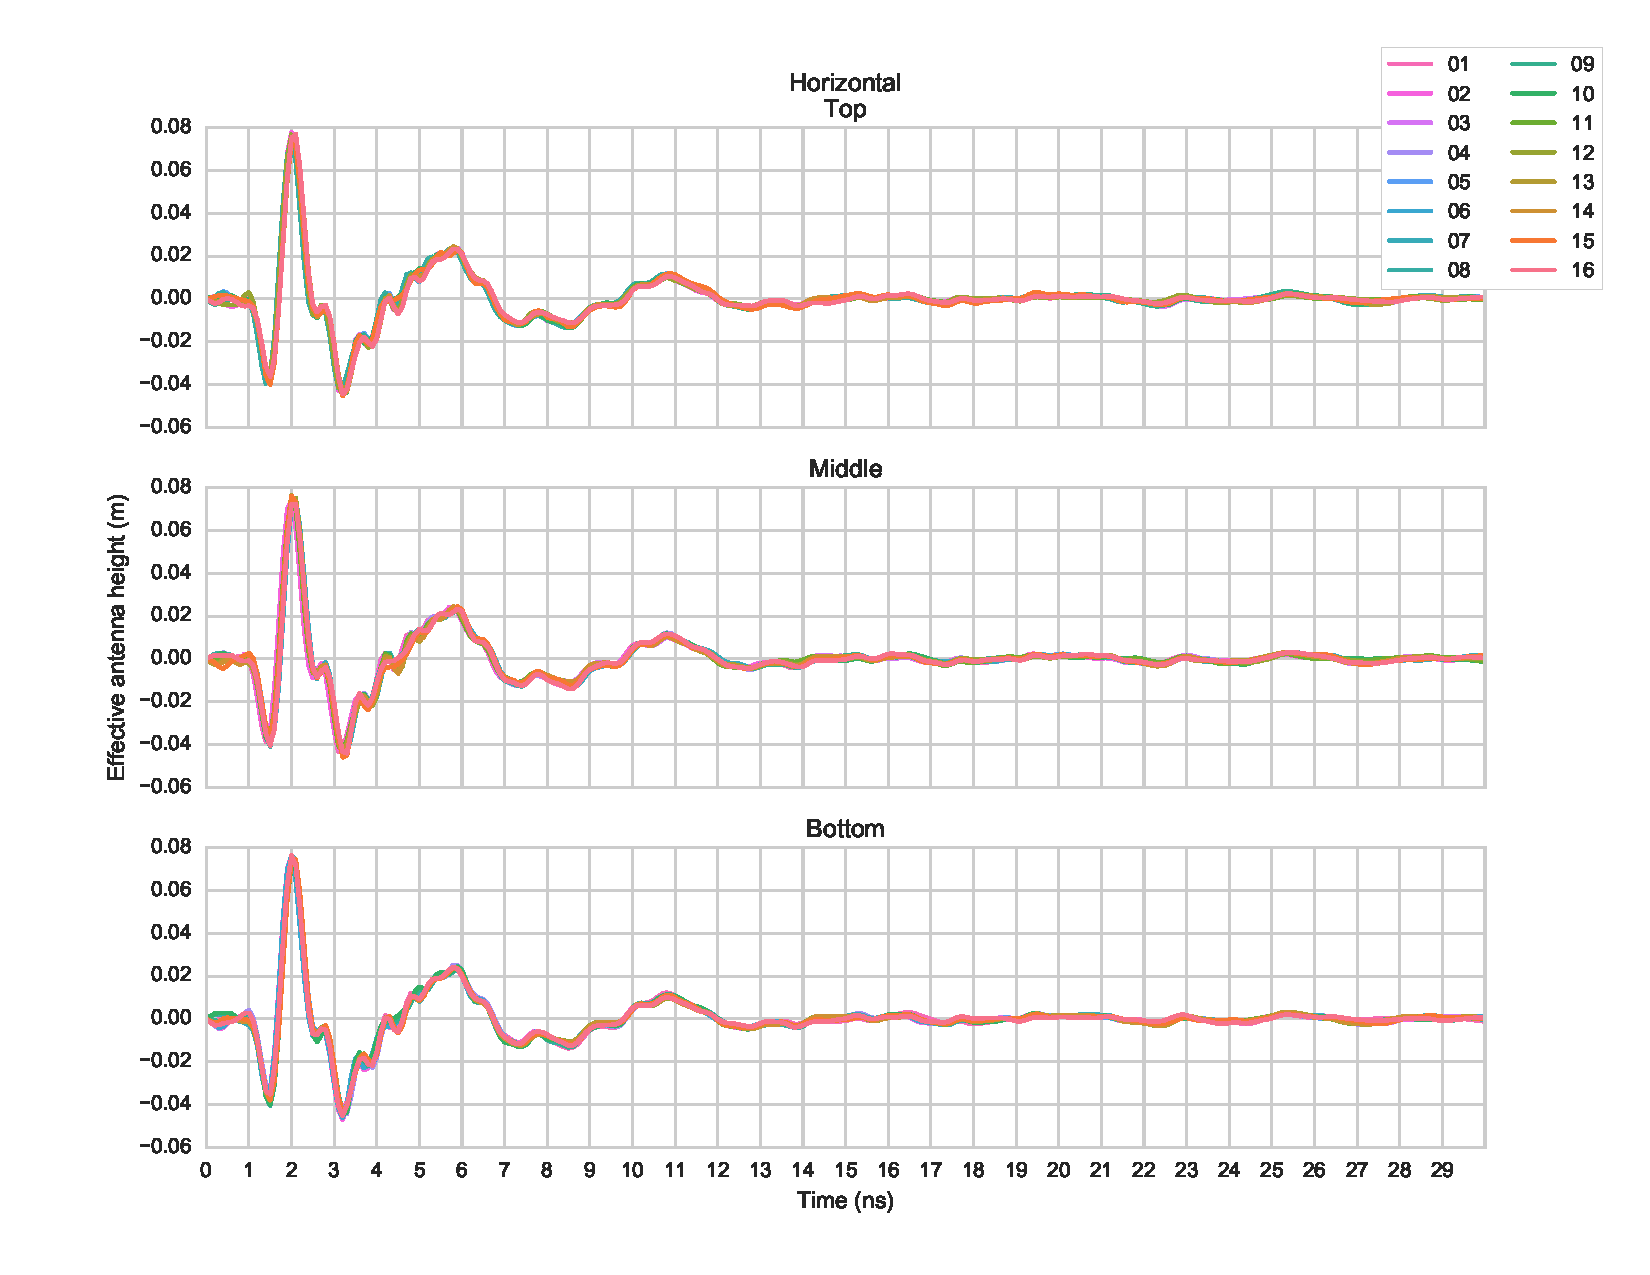
\includegraphics[width=1.5\textwidth]{../figures/antResponse_timeH} }
	\caption{Time domain impulse response of the horizontally oriented polarizations of the ANITA3 horn antennas.}
\label{fig:antResponse_timeH}
\end{figure}

\begin{figure}
\centering
\makebox[\textwidth]{%
	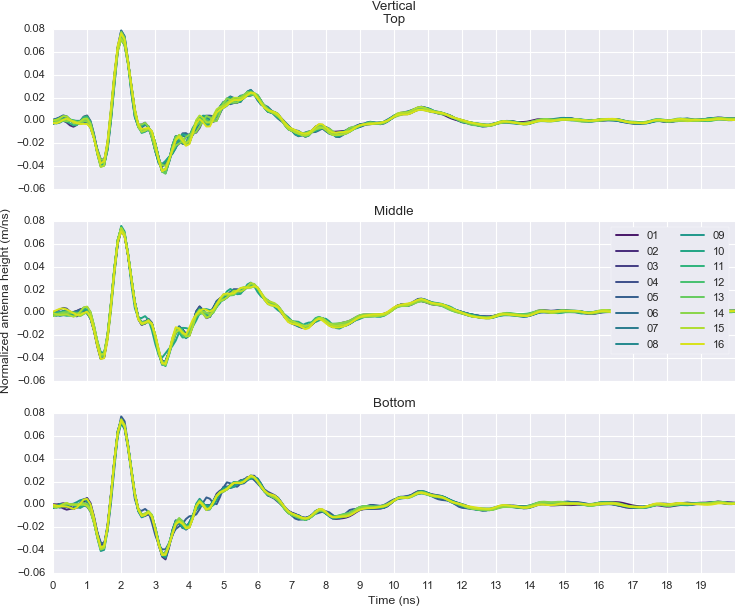
\includegraphics[width=1.5\textwidth]{../figures/antResponse_timeV} }
	\caption{Time domain impulse response of the vertically oriented polarizations of the ANITA3 horn antennas.}
\label{fig:antResponse_timeV}
\end{figure}

\begin{figure}
\centering
\makebox[\textwidth]{%
	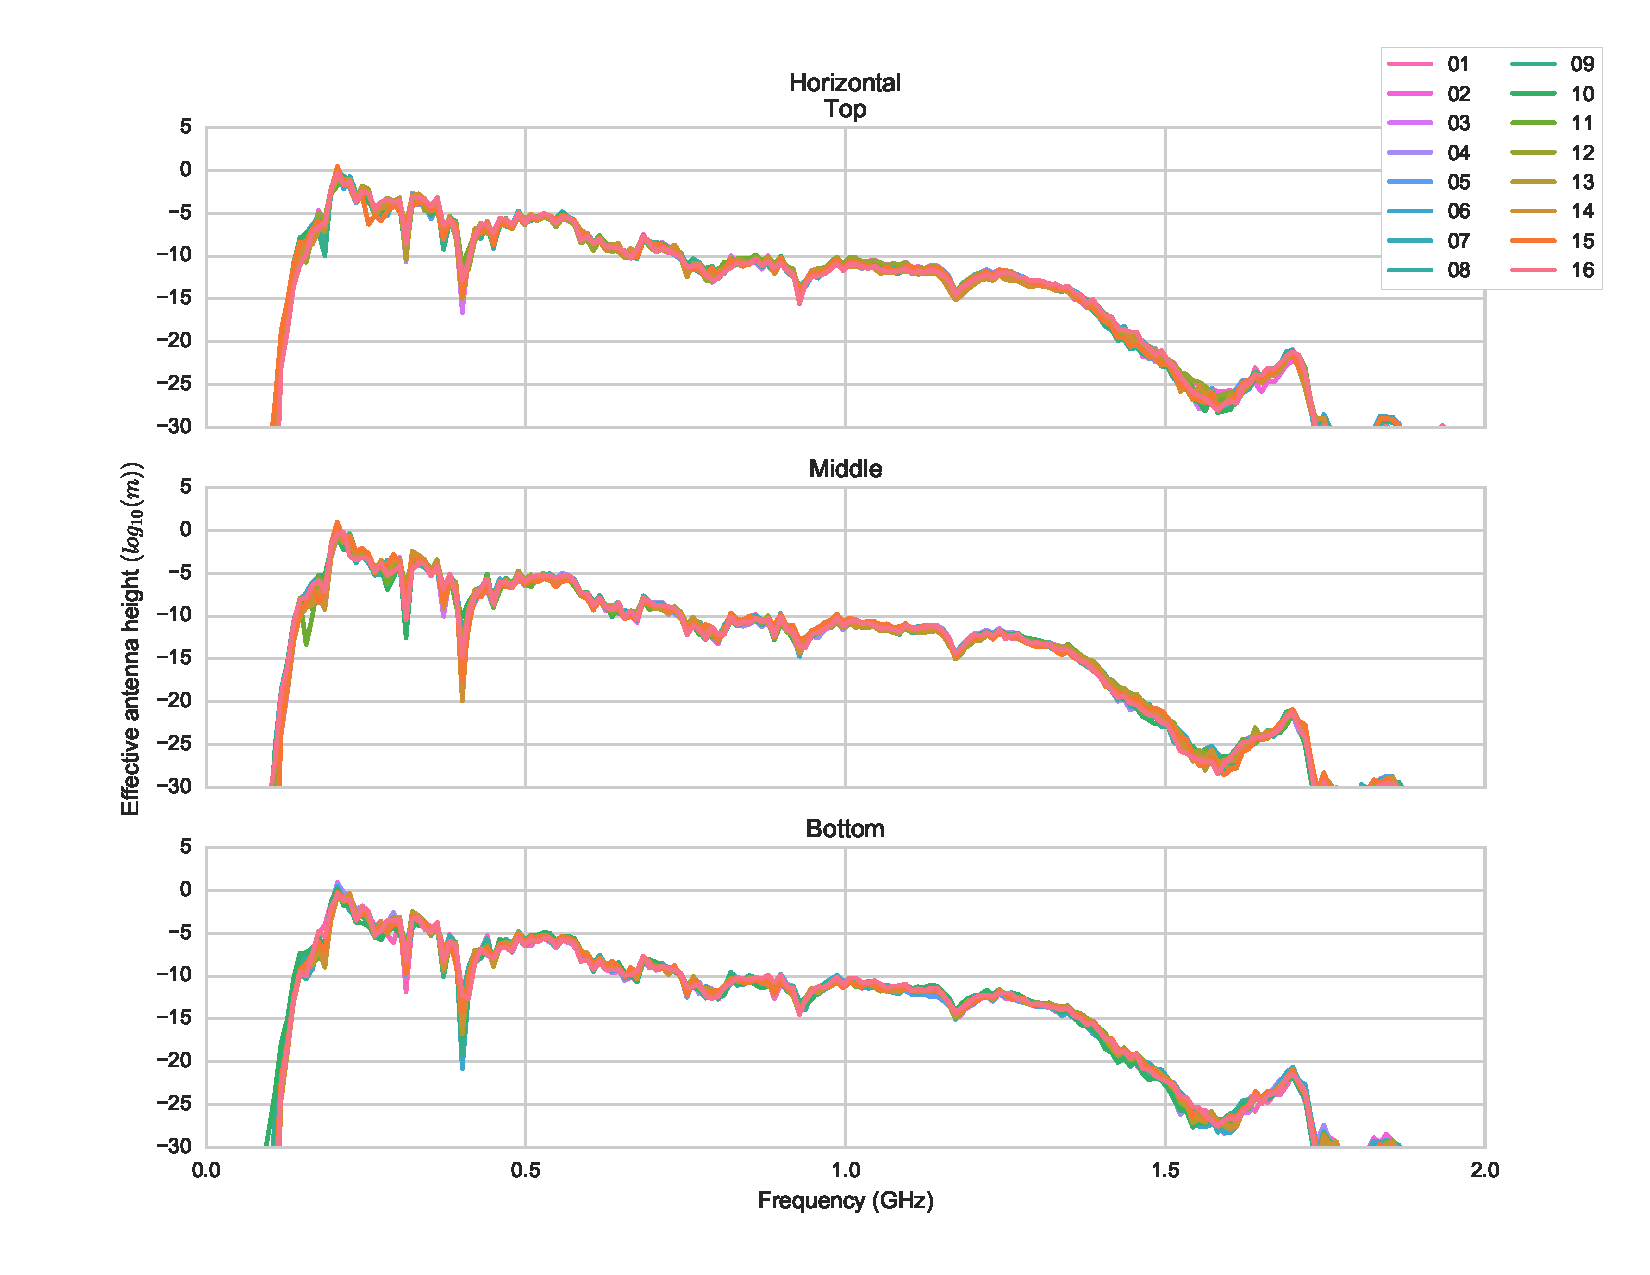
\includegraphics[width=1.5\textwidth]{../figures/antResponse_fftH} }
	\caption{Complex antenna height for the horizontally oriented polarizations of the ANITA3 horn antennas.}
\label{fig:antResponse_fftH}
\end{figure}

\begin{figure}
\centering
\makebox[\textwidth]{%
	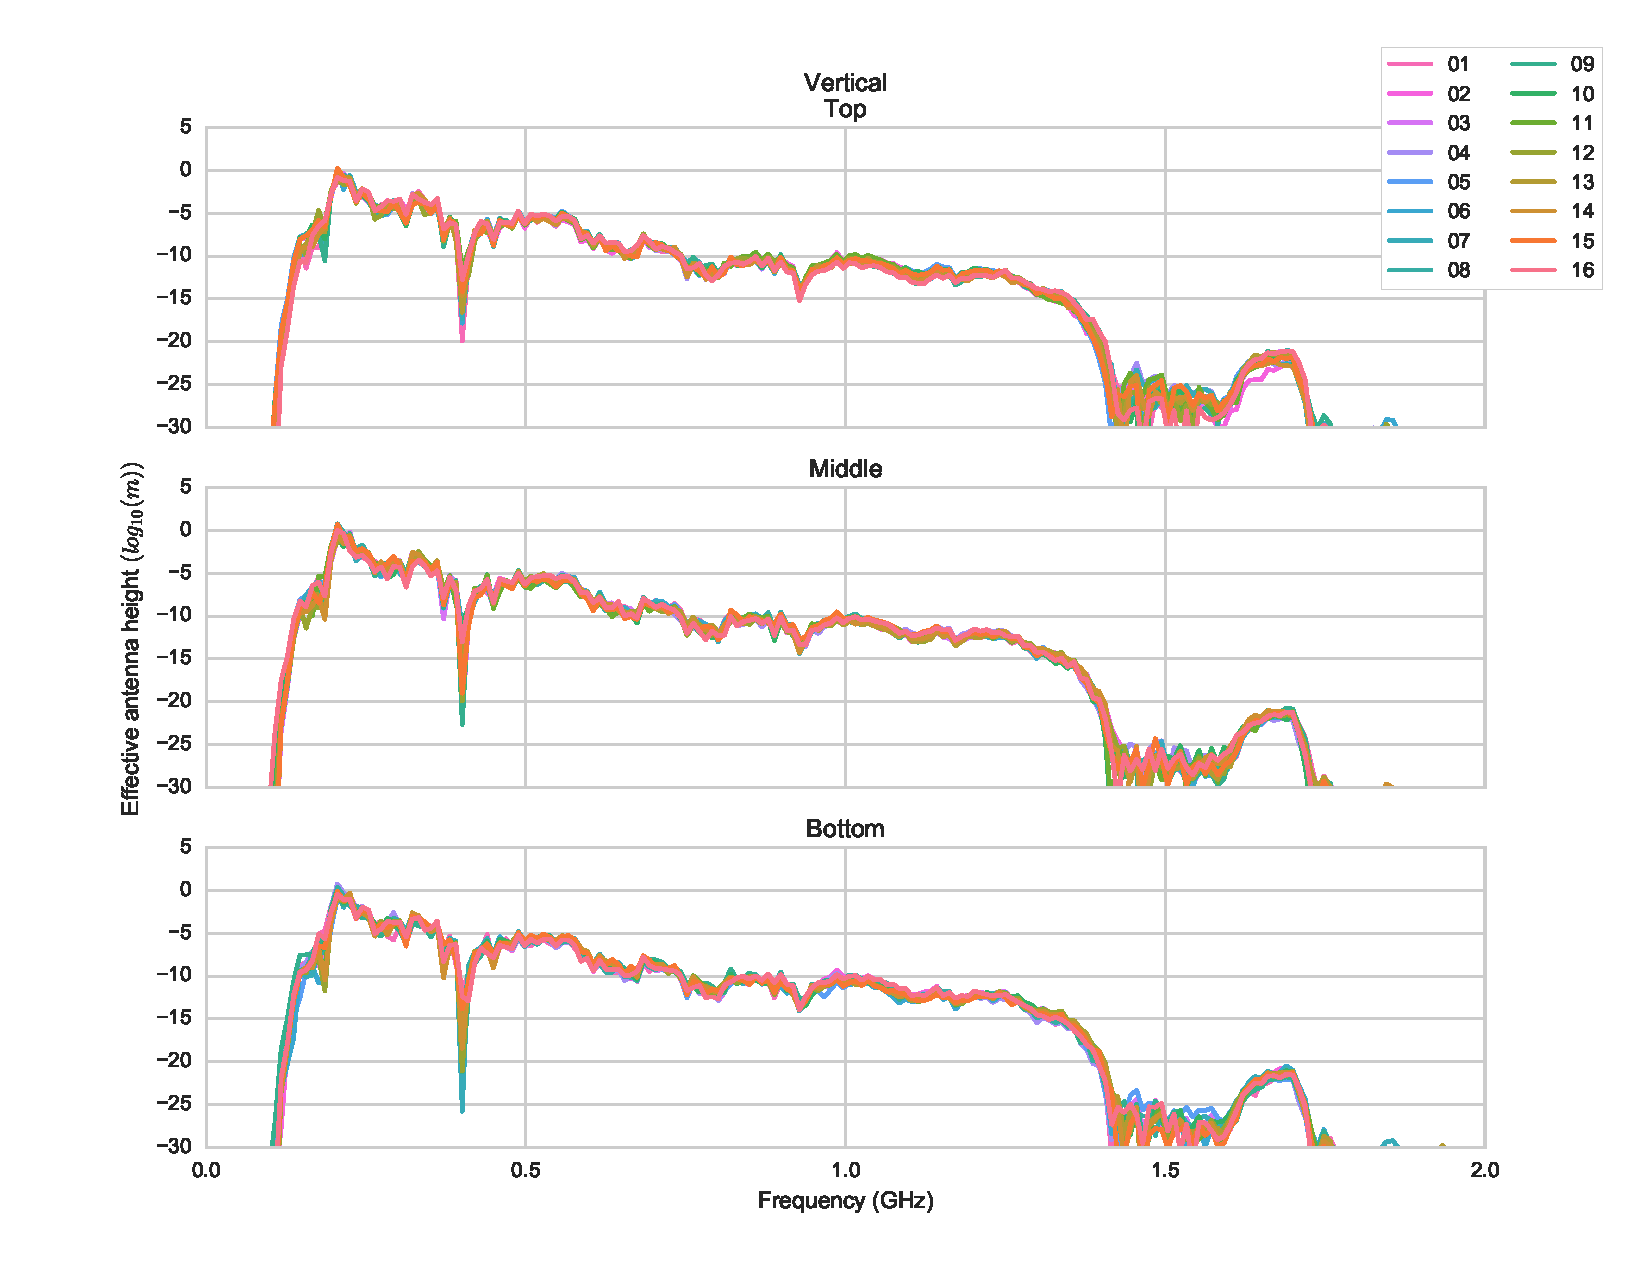
\includegraphics[width=1.5\textwidth]{../figures/antResponse_fftV} }
	\caption{Complex antenna height for the vertically oriented polarizations of the ANITA3 horn antennas.}
\label{fig:antResponse_fftV}
\end{figure}


\section{RF Signal Chain Impulse Response}
		
	\subsection{Measurements Summary}
		Measurements of each of the 96 signal chains flown in the ANITA3 instrument was done in Antarctica immediately preceding the flight.  To accomplish this, a broad band impulse was injected into each channel sequentially and measured by the on board flight electronics.  This signal was split and measured by a oscilloscope, providing an input and output reference signal with which we can compare to determine the full complex transfer function.  A diagram of the setup is seen in Figure \ref{fig:sigChainSetup}.


\begin{figure}
\makebox[\textwidth]{%
	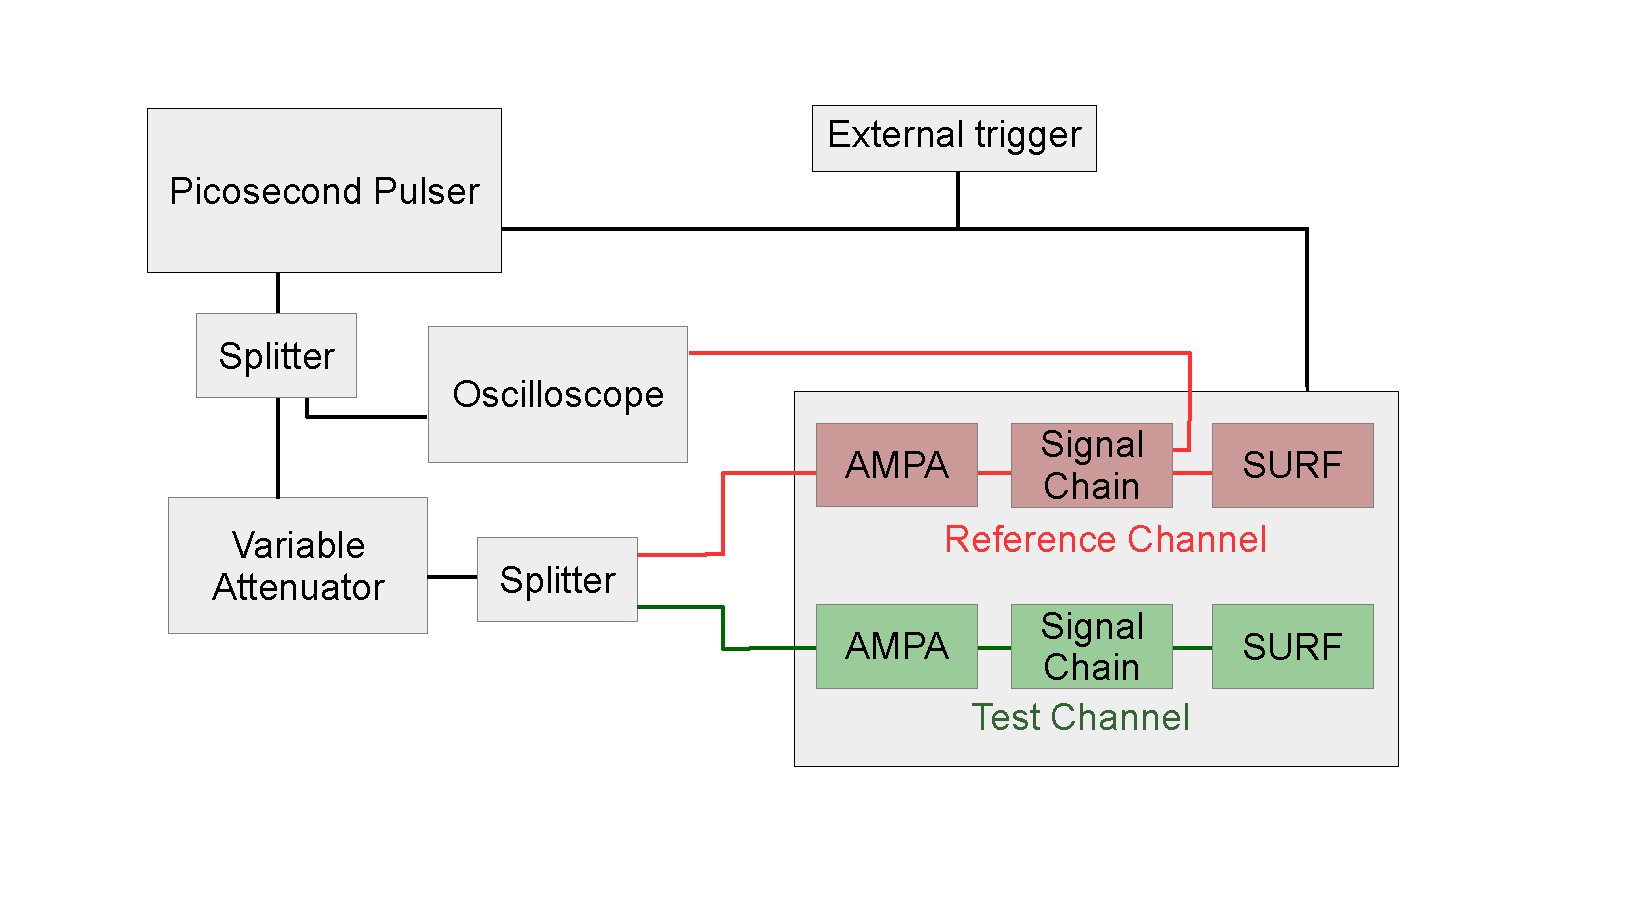
\includegraphics[width=1.5\textwidth]{../figures/antarctica14_calSetup} }
	\caption{A schematic of the pulse insertion calibration setup used immediately before flight with the full signal chain in Antarctica in 2014}
	\label{fig:sigChainSetup}
\end{figure}
			
	Note that the cables connecting the various elements of the calibration test setup are not present in the final flight configuration, and need to be measured and removed.
			

	\subsection{Expectation From Link Budget}
		Measurements of individual elements of the signal chain were taken prior to assembly and integration into the full signal chain.  These measurements can be combined to determine an expected hypothesis to which we can compare our final measured transfer function for each channel.  The averaged gains of each component are detailed in Table \ref{tab:linkBudget}
		
	\begin{figure}
		\begin{tabular}
	
		\end{tabular}
	\end{figure}

		
	\subsection{Complex Transfer Function}
		The full mathematical relationship between two waveforms that have traversed a non-linear signal network is called the complex transfer function, which I will denote with $h_{sig}(t)$ and it's Fourier transform equivalent, $\mathcal{H}_{sig}(f)$.  The relationships between a measured input signal $V_{in}(t)$ and output signal $v_{out}(t)$, and their respective Fourier transform equivalents $\mathcal{F}_{in}(f)$ and $\mathcal{F}_{out}(f)$, are shown in Equation \ref{eqn:ComplexTF}.
	
\begin{equation}
\begin{split}
V_{out}(t) = h_{sig}(t) \circ V_{in}(t) \\
\mathcal{F}_{out}(f) = \mathcal{H}_{sig}(f) \mathcal{F}_{in}(f) \\
\label{eqn:ComplexTF}
\end{split}
\end{equation}

The $\circ$ denotes a convolution operator.  The Fourier domain equivalent to convolution is complex multiplication, which can be seen in this equation pair.  Using these equations and the measurements of input and output digitized time domain waveforms we can determine the complex transfer function for each channel of the ANITA3 signal chain.

		

	\subsection{Methods and tools}
	
	
	\subsection{Results for Signal Chain Transfer Function}
		
	
	
	A variety of methods and tools are required to relate the different calibration data to each other to determine a final transfer function for the system.  Each of these has their own effect on the 


\section{Full Instrument Response}

	The final goal of determining the complex transfer functions for the antenna and signal chains is to relate measured ADC counts stored by the instrument into an incident electric field present on the payload.  The electric field is the true physics quantity being measured by the instrument, and a precise absolute value is desired.  Simulations of extensive air showers produced by terrestrial high energy particle interactions can generate electric field vector fields, which can be compared against our measurements only if we fully understand the full instrument response
	
	\subsection{Convolution of antenna and signal chain}
		The convolution of the antenna normalized complex height and the signal chain complex transfer function yield the following equation:
		
\begin{equation}
V_{meas}(t) = \sqrt{\frac{Z_{c}}{Z_{o}}}[h_{sig}(t) \circ h_{ant}(t) \circ E_{inc}(t)] \\
\label{eqn:fullConvolution}
\end{equation}

This can be simplified into a global complex instrument response, $h_{inst}(t)$:

\begin{equation}
\begin{split}
h_{inst}(t) = \sqrt{\frac{Z_{c}}{Z_{o}}}h_{sig}(t) \circ h_{ant}(t) \\ 
V_{meas}(t) = h_{inst}(t) \circ E_{inc}(t)
\end{split}
\label{eqn:instTF}
\end{equation}


\section{Magnitude Considerations and Absolute Response}
	
